\chapter{Организационно-экономический раздел}
\label{cha:econom}

Интернет-ссылки оформляются как \url{https://www.google.com/}. Ссылка на картинку, формулу и другие объекты происходит при помощи команды \verb|\ref|: см. рис. \ref{fig:example_fig_1}. На ссылку можно кликнуть и перейти к объекту, на который она ссылается. Ссылка может быть как до объекта, так и после него. Обычно, для удобства, идентификатор начинают с префикса <<\verb|fig:|>> для рисунков, <<\verb|tab:|>> для таблиц, <<\verb|eq:|>> для формул, для <<\verb|section:|>> для разделов, <<\verb|th:|>> для теорем и так далее. Пример ссылки на раздел: см. раздел \ref{cha:research}. 

По условиям ГОСТ-а, на каждую картинку и таблицу должна присутствовать в тексте хотя бы одна ссылка. Желательно рядом с картинкой. Ссылка должна быть оформлена в духе "{}В соответствии с рисунком (таблицей, разделом) 2"{}.

Информация об цитируемых источниках хранится в файлах формата \verb|*.bib|. В этом проекте есть пример такого файла \verb|references.bib|. Похож на формат \verb|json|, но им не является. Заполняйте как можно больше полей там. Сразу готовую запись можно получить прямо в Google Scholar или, часто, на страницах статей на других ресурсах (см. рис. \ref{fig:scholar}). Описание статей начинается с заголовка \verb|@article|, для источников других видов предусмотрены другие заголовки, например \verb|@online| для интернет-страниц.

\begin{figure}[ht]
    \centering
    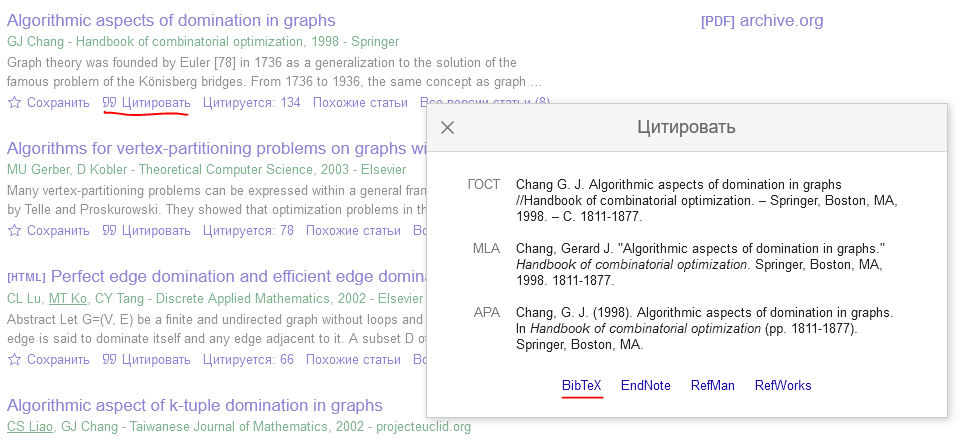
\includegraphics[scale=0.5]{res/img/scholar.png}
    \caption{Как получить bib-цитату на источник в Google Scholar.}
    \label{fig:scholar}
\end{figure}

Ссылка на источник происходит при помощи команды \verb|\cite|: \cite{duportail:alu}. В качестве единственного аргумента указывается идентификатор источника в одном из файлов \verb|*.bib|. Можно указать несколько источников: \cite{duportail:alu, husserl:pd, althusser:iia}, с \verb|\ref| так нельзя. В списке источников отображаются только те источники, на которых есть хотя бы одна ссылка. Если всё-же нужно что бы он там появился без единой ссылки, можно использовать команду \verb|\nocite| в любом месте программы, как под этим абзацем.

Вообще все ссылки кликабельны. Если ссылка неправильная, компилятор выдаст предупреждение, а ссылка будет выглядеть так: \textbf{??}.

\nocite{duportail:alu}
\nocite{althusser:iia}
\nocite{husserl:pd}
\nocite{husserl:sbe}
